\subsection{ElSe im Test}
\begin{frame}
\begin{figure}
	\centering
	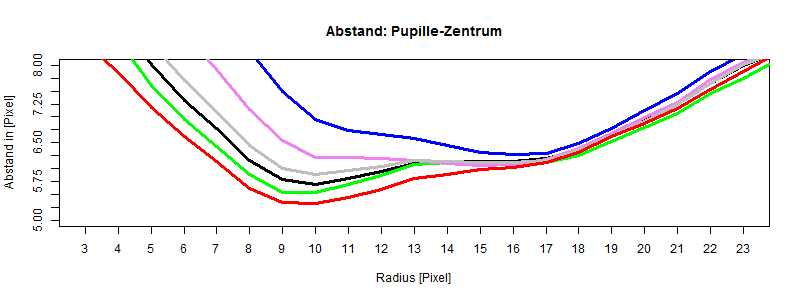
\includegraphics[width=\linewidth]{img_ElSe/Vergleich_A}
\end{figure}
Median-Abstand in Pixel des Zentrums der Pupille gegen die Veränderung des Radius des Filters.\\
Verfahren: Gleam (rot), Luminance (schwarz), Max (grün), Min (violett), New-Gleam (grau), Quadrat (blau)
\end{frame}
\begin{frame}
\begin{figure}
	\centering
	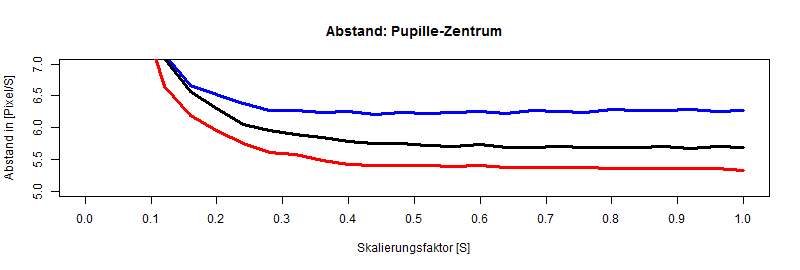
\includegraphics[width=0.8\linewidth]{img_ElSe/Vergleich_Scal_A}
	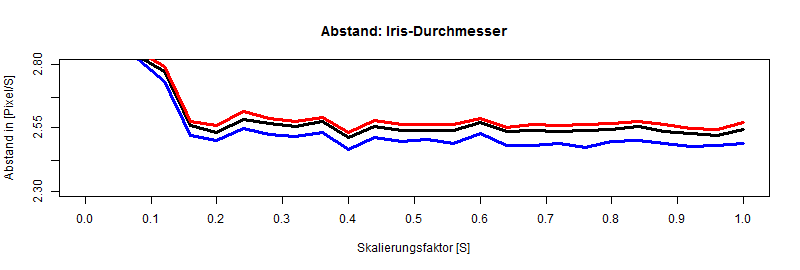
\includegraphics[width=0.8\linewidth]{img_ElSe/Vergleich_Scal_I}
\end{figure}
Abstand in Pixel zwischen der Berechnung und des Datensatzes bei verschiedenen Skalierungen.\\
Originaler durchschnittlicher Pupillendurchmesser 15 Pixel.\\
Gleam (rot), Luminance (schwarz),  Quadrat (blau)
\end{frame}
\subsection{OpenFace im Vergleich}
\begin{frame}
\begin{figure}
	\centering
	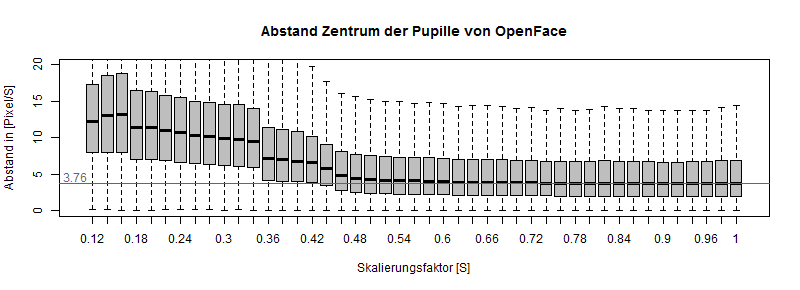
\includegraphics[width=0.8\linewidth]{img_ElSe/OpenFace_PC}
	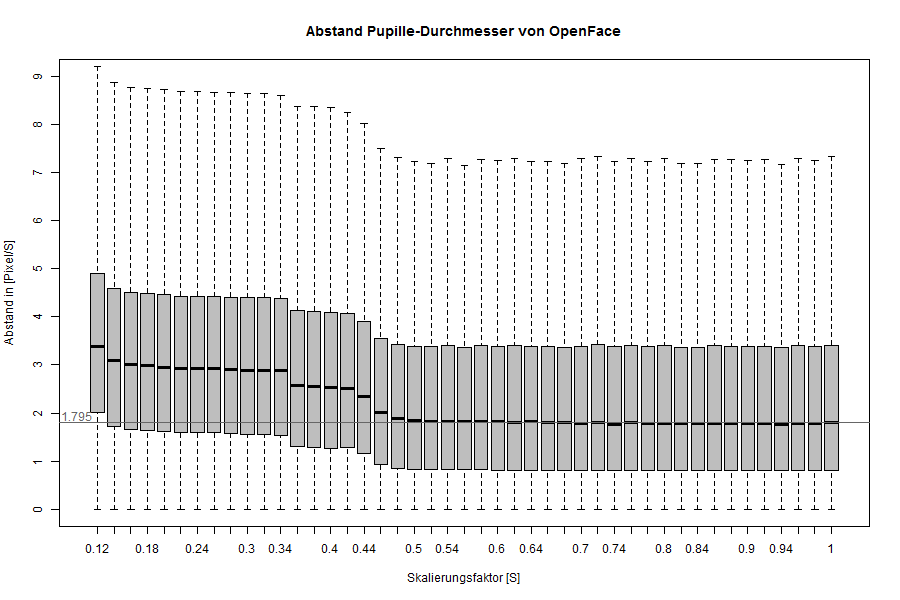
\includegraphics[width=0.8\linewidth]{img_ElSe/OpenFace_PW}
\end{figure}
Abstand in Pixel zwischen der Berechnung und des Datensatzes bei verschiedenen Skalierungen.\\
Originaler durchschnittlicher Irisdurchmesser 34 Pixel.\\
\end{frame}